%\documentclass{beamer}
\documentclass[handout]{beamer}
%\usetheme{Madrid} 
\usetheme{default}

%math fonts
\renewcommand\mathfamilydefault{\rmdefault}

%page numbers
\setbeamertemplate{footline}[page number]

\setbeamercovered{invisible}
\setbeamertemplate{navigation symbols}{} 
\usepackage{mathtools}
\usepackage{graphicx}
\usepackage{amsmath}
\usepackage{epstopdf}
\usepackage{color}


\title[Learning for Trajectory Tracking]{Gaussian Process Optimization based Learning for Trajectory Tracking}
\author{Okan Koc}
\institute[IDSC]
{
ETH Z\"urich \\
Applied Mathematics \\
\medskip
{\emph{koco@student.ethz.ch}}
}
\date{\today}

% Custom commands
\newcommand{\state}{\mathbf{x}} % used to denote the system states
\newcommand{\traj}{\mathbf{s}} % used to denote the points on the trajectory to be tracked
\newcommand{\sysInput}{\mathbf{u}} % used to denote the system inputs
\newcommand{\context}{\mathbf{c}} % used to denote contexts
\newcommand{\observations}{\mathbf{y}} % used for the observed output
% Set the paths where all figures are taken from:
\graphicspath{{Pictures/}}
\mathtoolsset{showonlyrefs} 
\newcommand{\includesvg}[1]{%
% \executeiffilenewer{#1.svg}{#1.pdf}%
% {inkscape -z -D --file=#1.svg %
% --export-pdf=#1.pdf --export-latex}%
 \input{#1.pdf_tex}%
}

\begin{document}
%
\begin{frame}
\titlepage
\end{frame}
%
\begin{frame}
\frametitle{Table of Contents}
\tableofcontents
\end{frame}
%
\section{Motivation}
%
\begin{frame}{Iterative Learning Control}
\begin{itemize}
\item Problem: Follow a trajectory under unknown repeating disturbances and model mismatch. \pause
\item Control inputs are adjusted at each iteration. \pause
	\begin{itemize}
	\item \emph{Feedforward} (open-loop) adjustment. \pause
	\end{itemize}
\item Not well generalized to different trajectories: \pause
	\begin{itemize}
	\item Not actually learning the \emph{dynamics}, \pause
	\item Instead learning to \emph{compensate} for the disturbances. \pause
	\end{itemize}
\item We develop another framework \pause
	\begin{itemize}
	\item To learn the dynamics \emph{during} trial runs, not \emph{between}. \pause
	\item To learn to generalize for different tasks.
	\end{itemize}
\end{itemize}
\end{frame}
%
\section{Gaussian Processes/Bandit Problems}
%
\begin{frame}{Gaussian Processes (GP)}
\begin{itemize}
\item Collection of dependent random variables $x$, any finite number of which has a joint Gaussian distribution \cite{GPbook}. \pause
\item Completely specified by a mean function $\mu(x)$ and a covariance (or kernel) function $k(x,x')$. \pause
\item From a Bayesian perspective defines a prior distribution over functions. \pause
\item Nonparametric regression: \pause
	\begin{itemize}
	\item No parameters to fix, \pause
	\item Kernel and mean function \emph{hyperparameters} to adjust the prior.
	\end{itemize}
\end{itemize}
\end{frame}
%
\begin{frame}{Gaussian Processes}
\begin{itemize}
\item Noisy observations $\observations_{N}$ at sample points $X$, \emph{update} the priors: \pause
\begin{align}
\mu_N{(x)} = \mu(x) + \mathbf{k}_N(x)^{\mathrm{T}}[\mathbf{K}_N + \sigma_{n}^{2}\mathbf{I}]^{-1}(\observations_N - \boldsymbol{\mu}_N) \\
k_N(x,x') = k(x,x') - \mathbf{k}_N(x)^{\mathrm{T}}[\mathbf{K}_N + \sigma_{n}^{2}\mathbf{I}]^{-1} \mathbf{k}_N(x') 
\end{align} 
\pause	
\item $\boldsymbol{\mu}_N = [\mu(x_1),\ldots,\mu(x_N)]^\mathrm{T}$ \pause
\item $\mathbf{k}_N(x) = [k(x_1,x),\ldots,k(x_N,x)]^\mathrm{T}$ \pause 
\item $\mathbf{K}_N = [k(x,x')]_{x,x' \in X} \succeq 0.$ \pause
\end{itemize}
\end{frame}
%
\begin{frame}{Gaussian Processes}
\begin{figure}
\center
\includegraphics[scale=0.30]{gp_regression.pdf}			
%\caption{GP Example}
\end{figure}
\end{frame}
%
\begin{frame}{Bandit Problems}
\begin{itemize}
\item Basic setting to solve the \emph{exploration-exploitation} dilemma. \pause
\item In the context of (stochastic) function optimization: \pause
	\begin{itemize}
	\item \emph{Exploration} of promising points in search space, \pause
	\item \emph{Exploitation} of the current optimum. \pause
	\end{itemize} 
\item Upper confidence bound (UCB) based algorithms solve the problem by constructing a confidence interval around each point. \pause
\item Regret analysis: \pause
	\begin{itemize}
	\item Instantaneous regret $r_{t} = f(x_{t}) - f(x^{*})$. \pause
	\item Cumulative regret $R_{T} = \sum_{t=1}^{T}r_{t}$. \pause
	\item \emph{No-regret}: $\lim_{T \to \infty}R_{T}/T = 0$.
	\end{itemize}
\end{itemize}
\end{frame}
%
\begin{frame}{GP-UCB}
\begin{itemize}
\item Main Idea: Interpolate over points not observed with a Gaussian Process. \pause
\item Sample at each time stage $t$ the following point: \pause
\begin{equation}
\sysInput_{t} = \operatorname*{arg\,min}_{\sysInput \in U}\mu_{t-1}(\sysInput) - \beta_{t}^{1/2}\sigma_{t-1}(\sysInput) \label{ucb}
\end{equation} \pause
\item Provably converges \cite{Krause1} to global minimum w.h.p. \pause
	\begin{itemize}
	\item Sublinear cumulative regret $R_{T} = \mathcal{O}^{*}(T^{1/2})$ implies no-regret.
%	\item For many commonly used covariance functions, \pause
%	\item If $f \sim \mathcal{N}(\mu(x),k(x,x'))$ for known mean and covariance functions.
	\end{itemize}
\end{itemize}
\end{frame}
%
\begin{frame}{Example}
\begin{figure}
\center
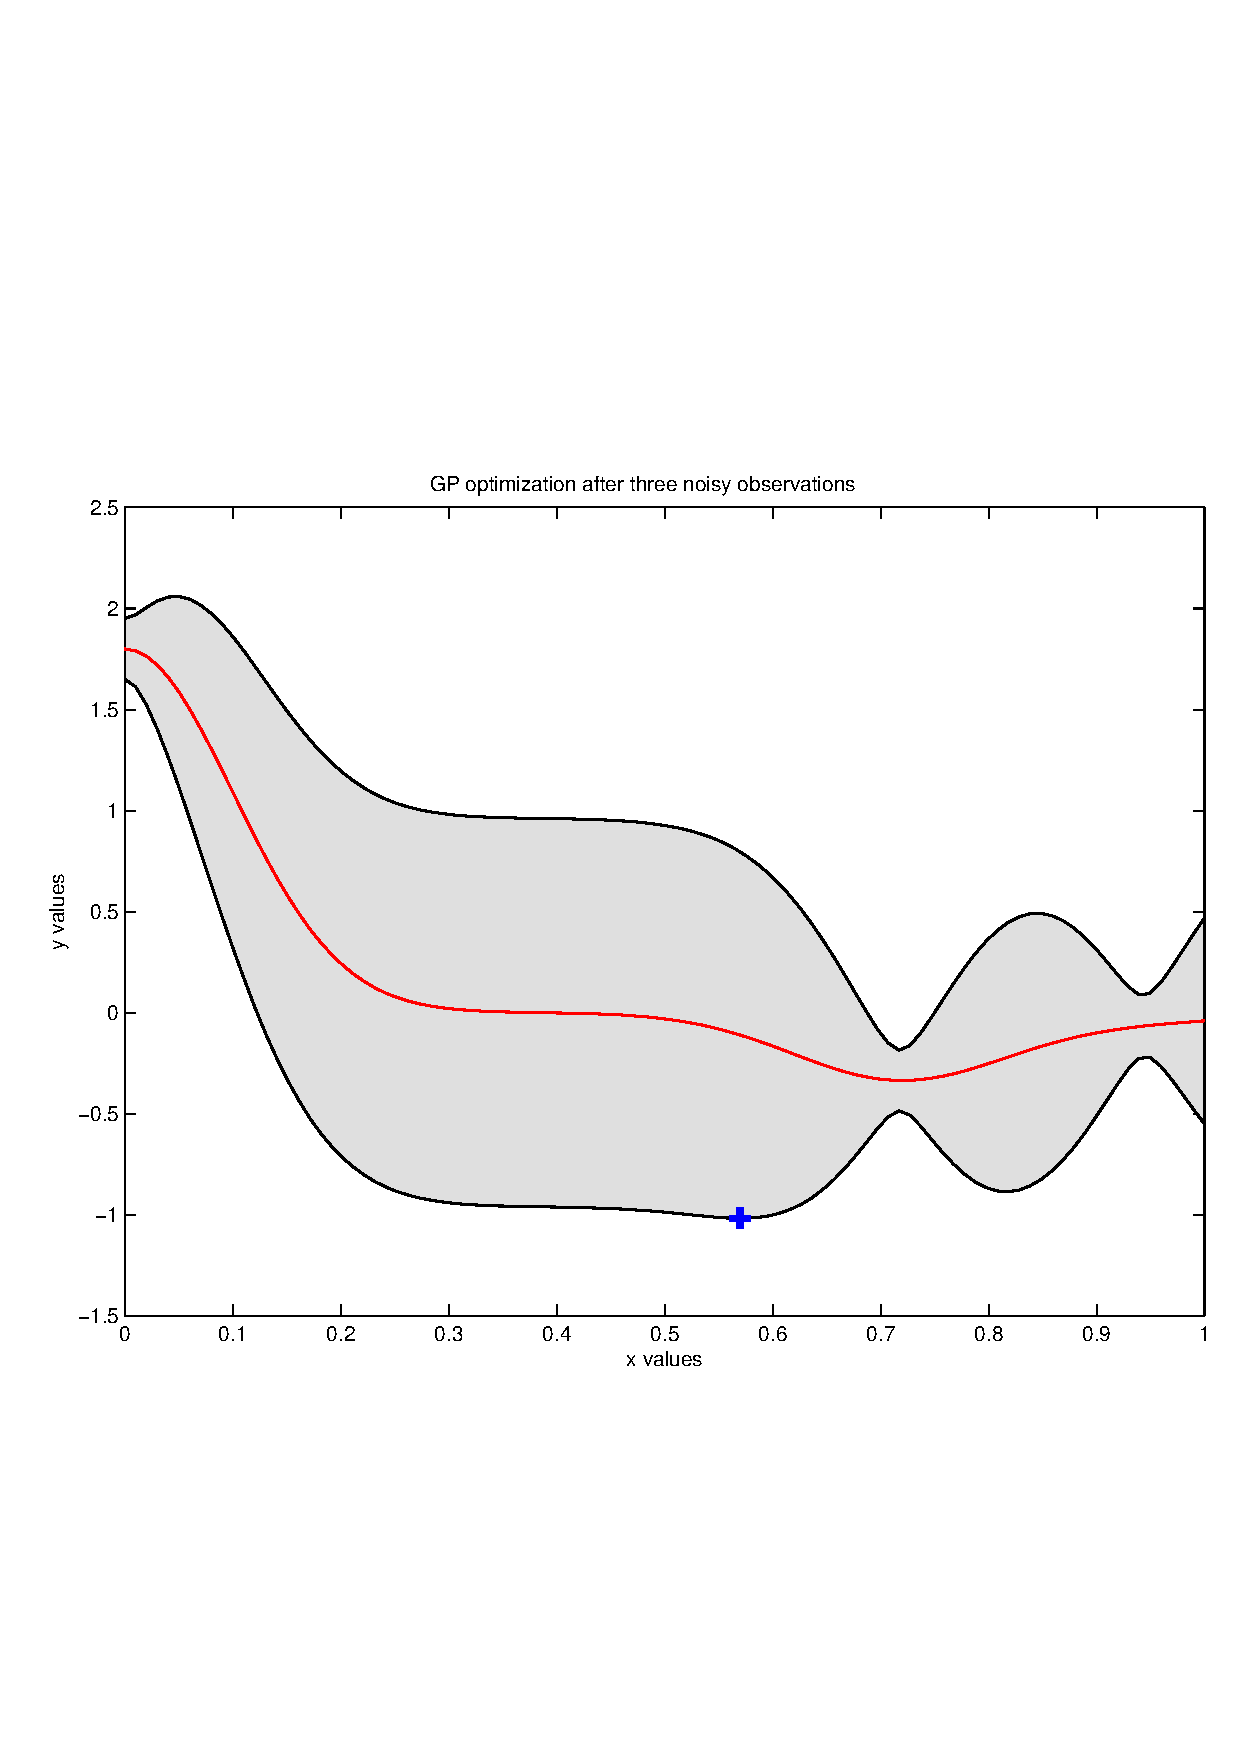
\includegraphics[scale=0.40]{test_gpucb1.pdf}			
\caption{GP-UCB optimization after 3 noisy observations}
\label{fig:gpucb1}
\end{figure}
\end{frame}
%
\begin{frame}{Example}
\begin{figure}
\center
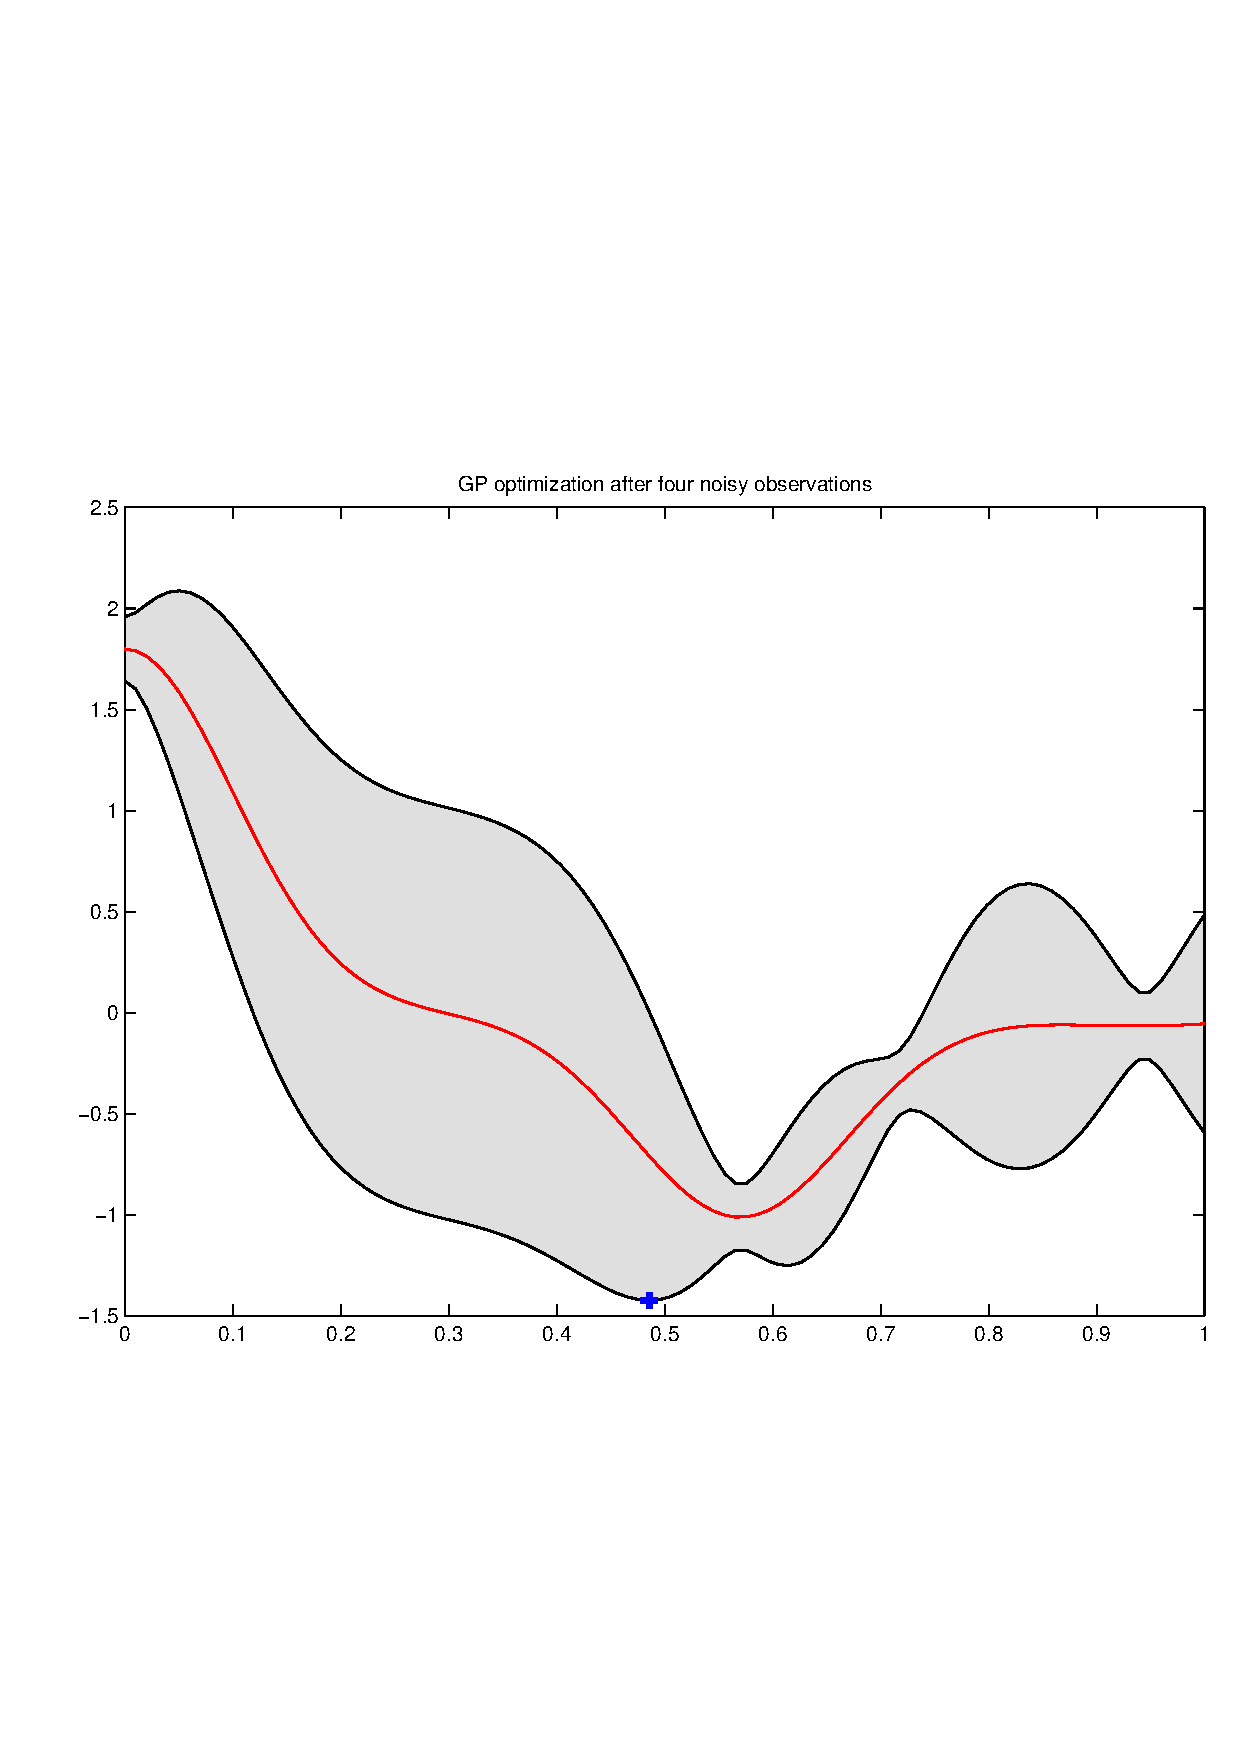
\includegraphics[scale=0.40]{test_gpucb2.pdf}			
\caption{GP-UCB optimization after 4 noisy observations}
\label{fig:gpucb2}
\end{figure}
\end{frame}
%
\begin{frame}{Contextual Bandits}
\begin{itemize}
\item Environment displays changing contexts, or states. \pause
\item CGP-UCB extends GP-UCB to contextual setting: \pause
\end{itemize}
\begin{equation}
\sysInput_{t} = \operatorname*{arg\,min}_{\sysInput \in U}\mu_{t-1}(\sysInput;\textcolor{blue}{\context_t}) - \beta_{t}^{1/2}\sigma_{t-1}(\sysInput;\textcolor{blue}{\context_t})
\end{equation}
\pause
\begin{itemize}
\item Provably converges \cite{Krause2} to global minimum for all $\context_t$ w.h.p. 
%	\begin{itemize}
%	\item For many commonly used covariance functions, \pause
%	\item If $f \sim \mathcal{N}(\mu(x),k(x,x'))$, $x = (\sysInput, \context)$ for known mean and covariance functions.
%	\end{itemize}
\end{itemize}
\begin{figure}
\center
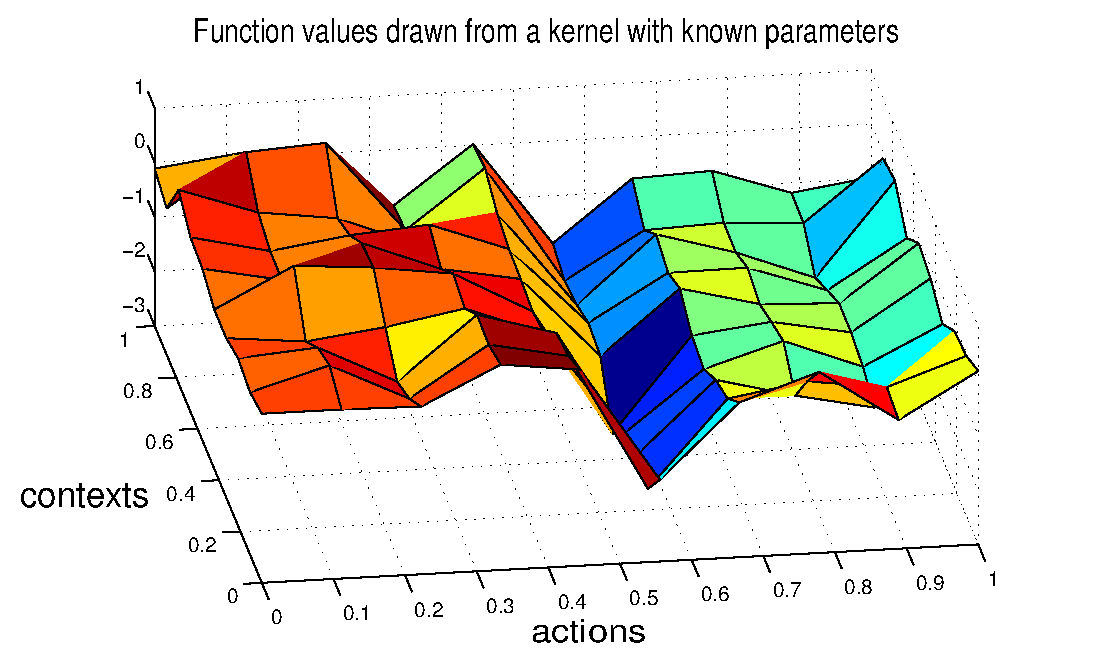
\includegraphics[scale=0.30]{test_fnc.eps}			
\caption{Function over $x = (\sysInput, \context)$}
\end{figure}
\end{frame}
%
\section{Methodology}
%
\begin{frame}{Problem Setting}
\begin{itemize}
\item Discrete time trajectory tracking objective: \pause
\end{itemize}
\begin{equation*}
\begin{aligned}
& \underset{u}{\text{minimize}}
& & \sum_{k \in \{h,2h,\ldots,Th\}} (\state_{k} - \traj_{k})^{\mathrm{T}}Q(\state_{k} - \traj_{k}) \\
& \text{subject to}
& & \state_{k+1} = \mathbf{f}(\state_k,\sysInput_k)
\end{aligned}
\end{equation*}
\pause
\begin{itemize}
\item $\mathbf{f}$ is not known very well! \pause
\item Proposed method: \pause
	\begin{enumerate}
	\item Learn the stage costs $\|\state_{k} - \traj_{k}\|_{Q}^{2}$ \pause (TBD)
	\item and  simultaneously track the trajectory
	\end{enumerate}
\end{itemize}
\end{frame}
%
\begin{frame}{Learning}
\begin{itemize}
\item We don't have $\mathbf{f}$ but we have $\mathbf{f}_{\mathrm{nom}}$! \pause
\item We can boost CGP-UCB with the nominal model: \pause
\end{itemize}
\begin{align}
\sysInput_{k} &= \operatorname*{arg\,min}_{u \in U(k)} \left\lbrace  \textcolor{blue}{\|\hat{\state}_{k+1} - \traj_{k+1}\|_{Q}^{2}} \right. 		+ \mu_{k-1}(\sysInput;\context_{k}) - \beta_k^{1/2}\sigma_{k-1}(\sysInput;\context_{k}) \rbrace \\
\hat{\state}_{k+1} &= \mathbf{f}_{\mathrm{nom}}(\state_k,\sysInput_k)
\end{align}
\begin{itemize}
\item Stage cost predicted by nominal model acts as a \emph{prior mean}. \pause
\item Context: $\state_{k} \times \traj_{k+1} \in C$
\end{itemize}
\end{frame}
%
\begin{frame}{Learning}
\begin{itemize}
\item Stage cost difference $\delta J_{k}$:  \pause
\begin{align}
\delta J_{k} &= \|\state_{k+1} - \traj_{k+1}\|_{Q}^{2} - \|\hat{\state}_{k+1} - \traj_{k+1}\|_{Q}^{2} \\
\delta J_{k} &: (\state_k, \traj_{k+1}; \sysInput_k) \mapsto \delta f^{\mathrm{T}} Q \delta f + 2(\hat{\state}_{k+1} - \traj_{k+1})^{\mathrm{T}} Q \delta f  \\
\delta f &:= \mathbf{f}(\state_k,\sysInput_k) - \mathbf{f}_{\mathrm{nom}}(\state_k,\sysInput_k)
\end{align}
\pause
\item After learning, \pause 
	\begin{itemize}
	\item Roll-out stage costs as in MPC for more stable tracking. \pause
	\end{itemize}
\item But we want to show convergence during learning!
\end{itemize}
\end{frame}
%
\begin{frame}{Tracking}
\begin{itemize}
\item Myopic policy! \pause
	\begin{itemize}
	\item Problem: $\traj_{k+1}$ not feasible if far away. \pause
	\item Solution: Make it feasible! \pause
	\end{itemize}
\item With a guiding oracle, we can show asymptotic convergence w.h.p. (TBD) \pause
\item $\state^{\mathcal{O}}_{k+1} = \mathcal{O}(\state(k), \traj(k+1), \ldots, \traj(k+T))$ \pause
\end{itemize}
\begin{figure}
	\centering
	\def\svgwidth{0.4\columnwidth}
	\includesvg{Pictures/oracle}
	\caption{Illustration of an oracle}
\end{figure}
\end{frame}
%
\begin{frame}{Oracle}
\begin{itemize}
\item Oracle $\mathcal{O}$ acts as a magnet around the trajectory.  \pause
\item If $\mathcal{O}$ can compute asymptotically converging trajectories: $\lim_{T \to \infty} d(\state_{k+1}^{\mathcal{O}},\traj_{k+1}) = 0$ \pause
\item If $\mathcal{O}$ incurs over time $T$ sublinear cumulative regret \pause
	\begin{itemize}
	\item $r_{k}^{\mathcal{O}} = \min_{u \in U(k)} d^{2}(\state_{k+1}(u),\state_{k+1}^{\mathcal{O}})$ \pause
	\end{itemize}
\item Then asymptotic convergence w.h.p. \pause
\end{itemize}
\begin{figure}
	\centering
	\def\svgwidth{0.4\columnwidth}
	\includesvg{Pictures/oracle}
	\caption{Illustration of an oracle}
\end{figure}
\end{frame}
%
\section{Results}
%
\begin{frame}{Results}
\begin{itemize}
\item Wind disturbance during quadrocopter operation. \pause
\item 2D Quadrocopter dynamics modified as follows: \pause
\end{itemize}
\begin{equation}
\begin{aligned}
\ddot{y} &= -f_{\mathrm{coll}} \sin\phi + P_{wind} A sin(\theta + \phi) cos \theta \\
\ddot{z} &=  f_{\mathrm{coll}}\cos\phi - g + P_{wind} A sin(\theta + \phi) sin \theta \\
\dot{\phi} &= \omega_{x}
\end{aligned}
\end{equation}
\begin{figure}
\center
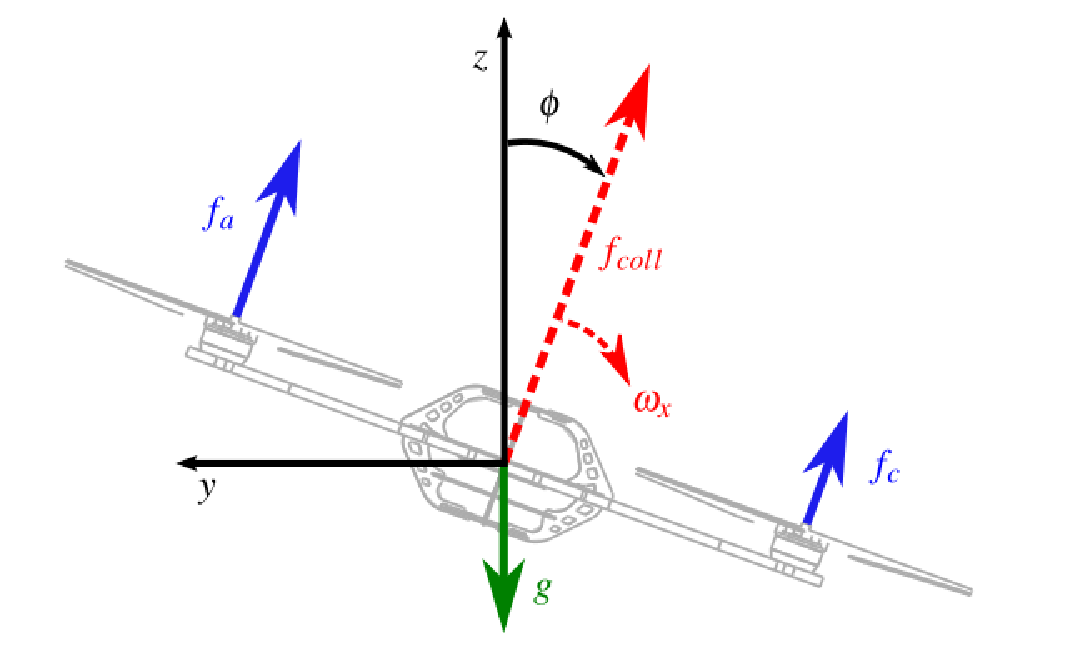
\includegraphics[scale=0.25]{quadrocopter}			
\caption{2D Quadrocopter model}
\end{figure}
\end{frame}
%
\begin{frame}{Results}
\begin{itemize}
\item CGP-UCB Result: \pause
\end{itemize}
\begin{figure}
\center
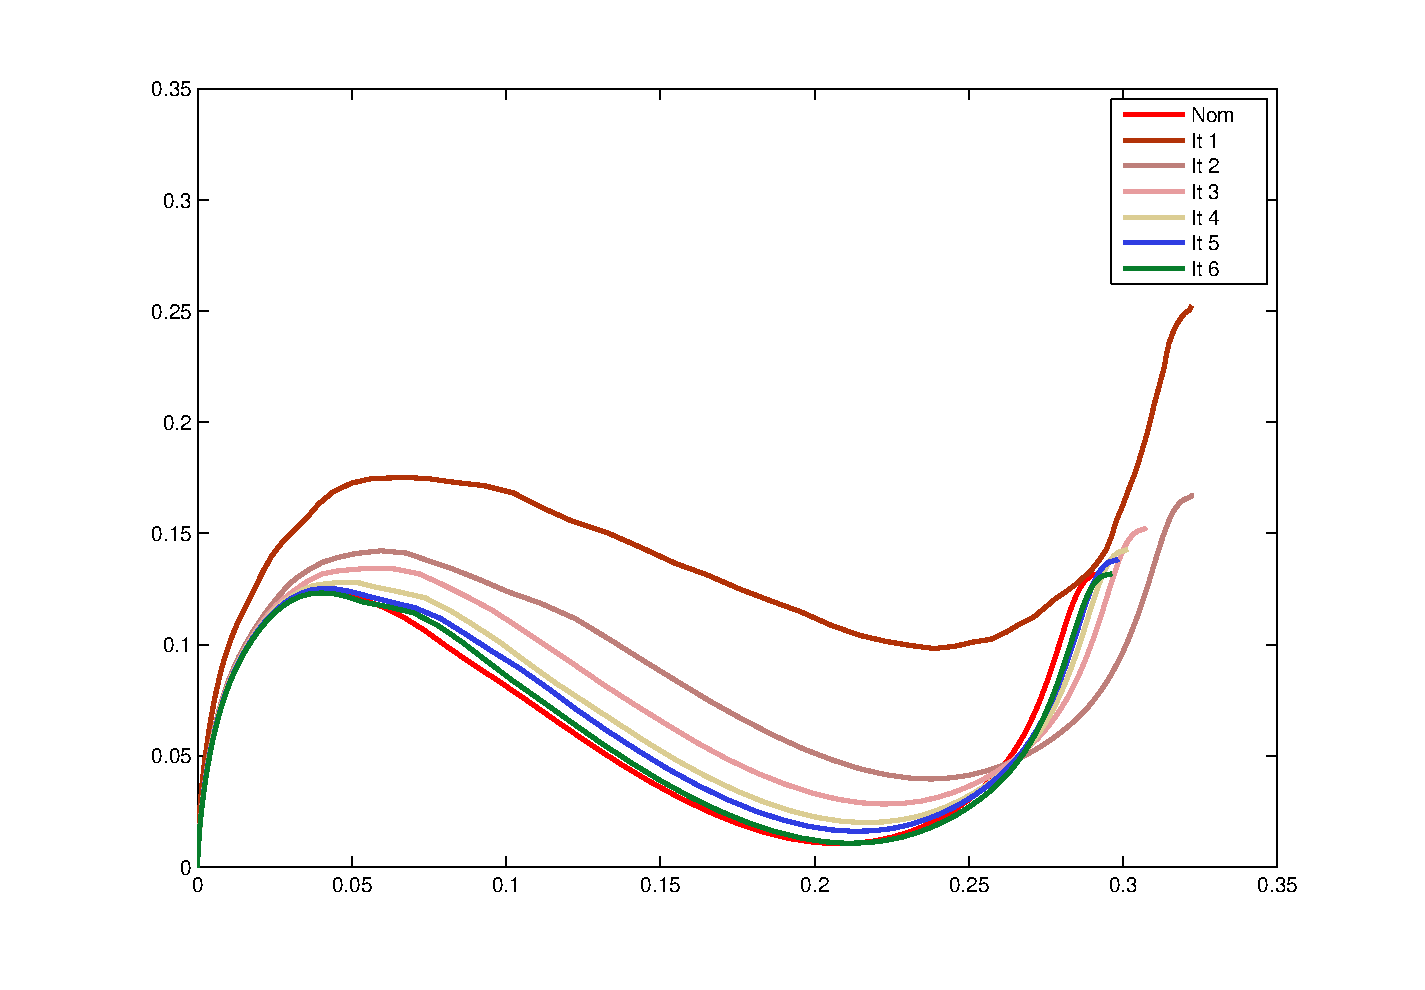
\includegraphics[scale=0.40]{CGPUCBwind_yz}			
\caption{CGP-UCB over iterations}
\end{figure}
\end{frame}
%
%\begin{frame}{Results B}
%\begin{itemize}
%\item Badly-modeled actuator: \pause
%\end{itemize}
%\begin{equation}
%\begin{aligned}
%\ddot{y} &= -f_{\mathrm{coll}}(1+k)\sin\phi \\
%\ddot{z} &=  f_{\mathrm{coll}}(1+k)\cos\phi - g\\
%\dot{\phi} &= \omega_{x}
%\end{aligned}
%\end{equation}
%\end{frame}
%
\begin{frame}{Transfer Learning}
\begin{itemize}
\item Transfer learning over 2 different trajectories
\end{itemize}
\begin{figure}
\center
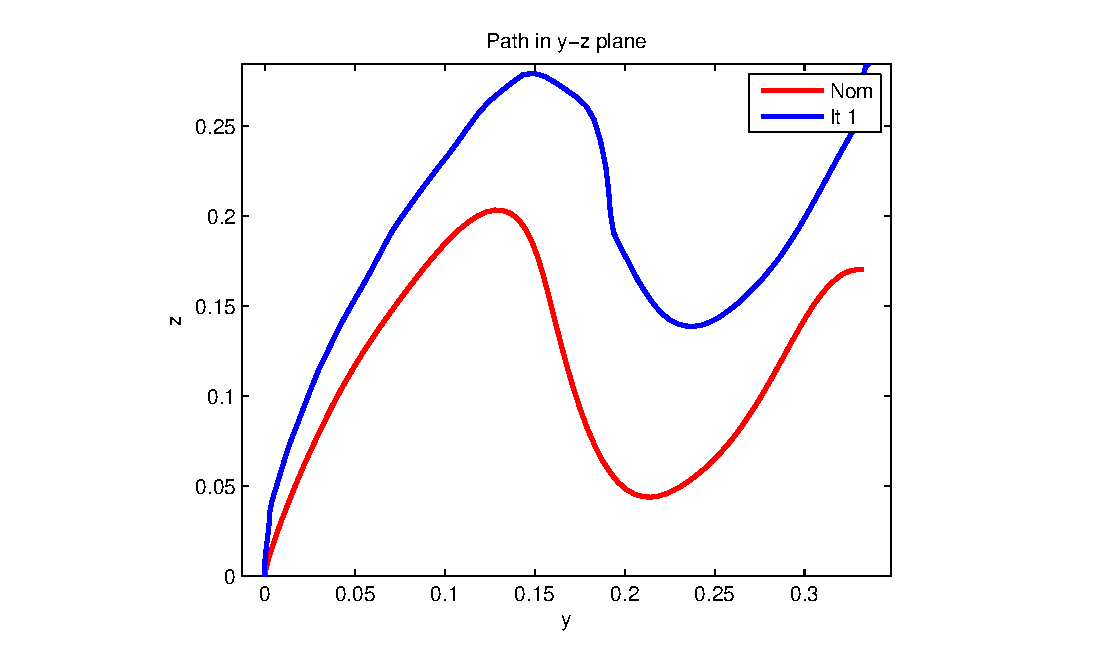
\includegraphics[scale=0.40]{transfer_learning0.eps}			
\caption{1st Iteration over initial trajectory}
\end{figure}
\end{frame}
%
\begin{frame}{Transfer Learning}
\begin{figure}
\center
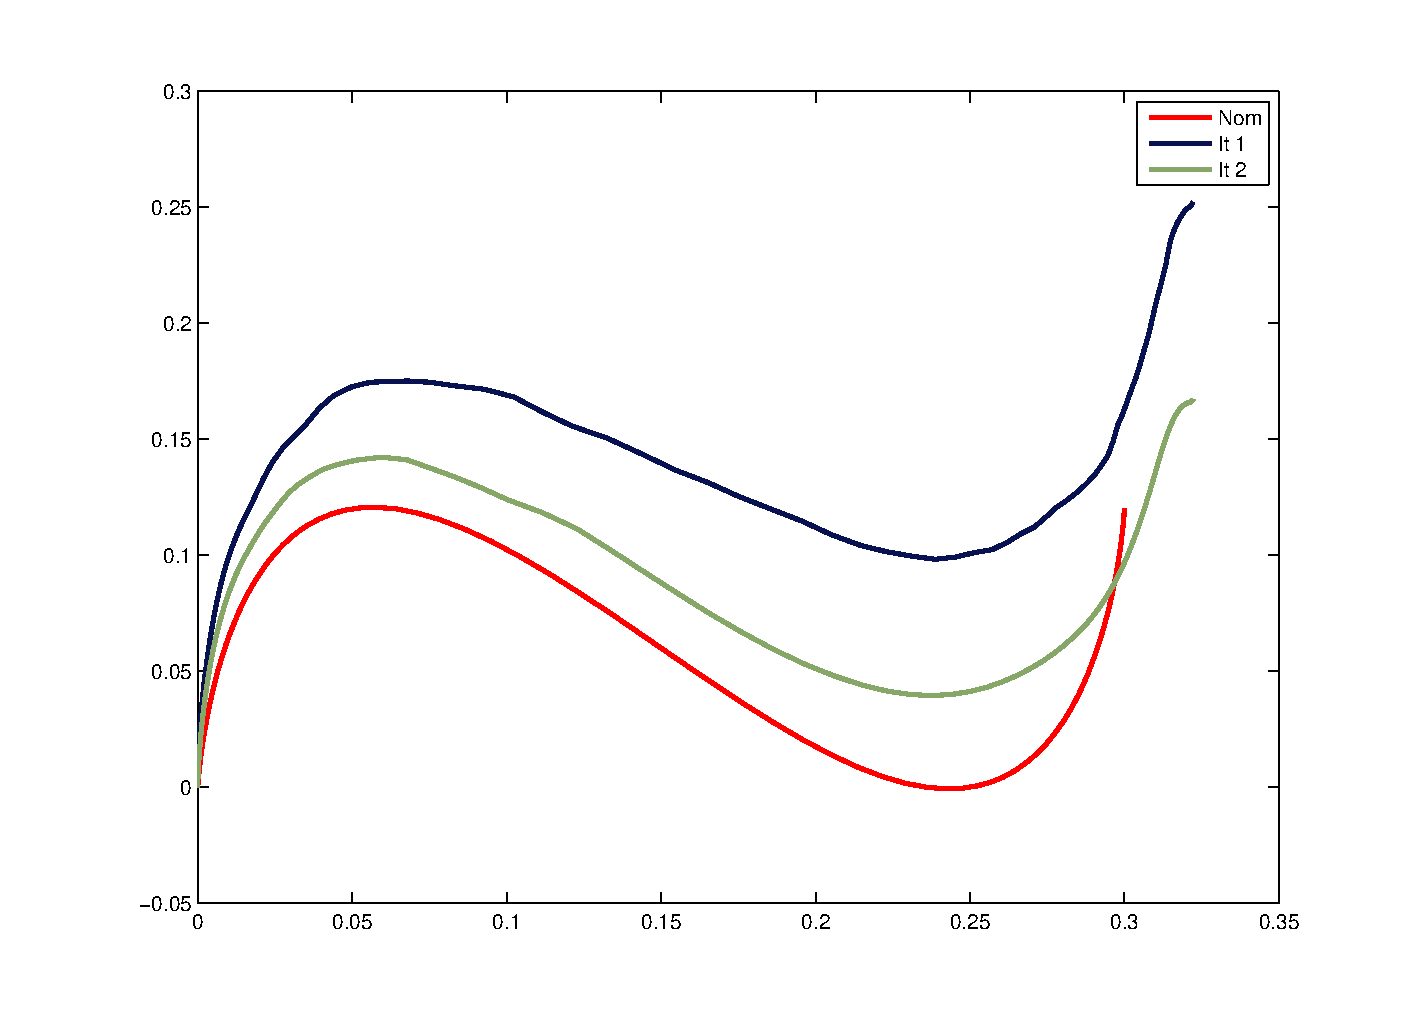
\includegraphics[scale=0.20]{transfer_learning1.eps}			
\caption{2 Iterations over second trajectory}
\end{figure}
\begin{figure}
\center
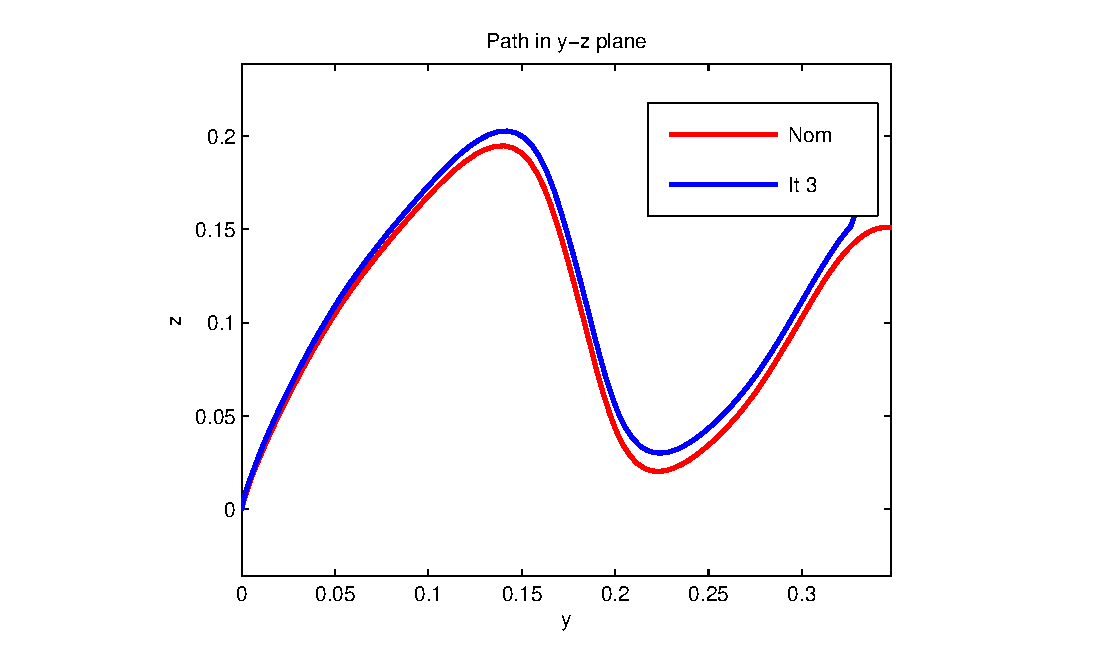
\includegraphics[scale=0.20]{transfer_learning2.eps}			
\caption{3rd Iteration over initial trajectory}
\end{figure}
\end{frame}
%
\section{Conclusions / Future Work}
%
\begin{frame}{Conclusion}
\begin{itemize}
\item We have demonstrated the performance of CGP-UCB in: \pause
	\begin{enumerate}
	\item Learning unknown dynamics, \pause
	\item Trajectory tracking, \pause
	\item Knowledge transfer between different trajectories. \pause
	\end{enumerate}
\item We solve the exploration-exploitation problem by: \pause
	\begin{enumerate}
	\item Exploring new control inputs when the uncertainty of that input is high enough, \pause
	\item Exploiting the learned dynamics (the mean value).
	\end{enumerate}
\end{itemize}
\end{frame}
%
\begin{frame}{Future Work}
\begin{itemize}
\item Effect of hyperparameter-mismatch on learning and tracking performance, \pause
\item Adaptive hyperparameter-estimation in complex environments, \pause
\item Perturbation analysis of optimization problems, \pause
\item Actual implementation on a robotic manipulator, \pause
\item Approximate Dynamic Programming: decomposition into a greedy learning step CGP-UCB and a planning step $H$.
\end{itemize}
\end{frame}
%
\begin{frame}[allowframebreaks]{References}
\def\newblock{\hskip .11em plus .33em minus .07em}
\bibliographystyle{alpha}
\bibliography{myReferences} % file name of the bibtex
\end{frame}
%
\begin{frame}
\centerline{Thank you for listening!}
\end{frame}
% Appendix
\appendix
%
\section{Kernels}
%
\begin{frame}{Kernels}
\begin{itemize}
\item Some commonly used examples of kernels: \pause
	\begin{enumerate}
	\item Squared exponential: $k(x,x') = \exp(-\frac{1}{2}(x-x')^{\mathrm{T}}\Lambda^{-1}(x-x'))$ \pause
	\item Linear: $k(x,x') = x^{\mathrm{T}}\Lambda^{-1}x'$ \pause
	\end{enumerate}
\item Composite kernels for $x = (\context, \sysInput)$: \pause
	\begin{enumerate}
	\item Tensor product: $k(x,x') = k_c(\context, \context')k_u(\sysInput, \sysInput')$ \pause
	\item Direct sum: $k(x,x') = k_c(\context, \context') + k_u(\sysInput, \sysInput')$
	\end{enumerate}
\end{itemize}
\end{frame}
%
\section{Estimation}
%
\begin{frame}{Maximum Likelihood Estimation}
\begin{itemize}
\item $\observations$ values are drawn from a Gaussian multivariate distribution. \pause
\item Negative log likelihood: \pause
\end{itemize}
\begin{equation}
\textbf{nll} = - \log \frac{1}{(2\pi^{N/2})|K_{\theta}|^{1/2}}e^{-(\observations - \mathbf{\mu})^{\mathrm{T}}K_{\theta}^{-1}(\observations - \mathbf{\mu})}
\end{equation}
\pause
\begin{equation}
\textbf{nll} = \frac{N}{2}\log(2\pi) + \underbrace{\frac{1}{2}\log|K_{\theta}|}_{\text{complexity penalty}} + \underbrace{(\observations - \mathbf{\mu})^{\mathrm{T}}K_{\theta}^{-1}(\observations - \mathbf{\mu})}_{\text{data fit}}
\end{equation}
\end{frame}
%
\section{Control-Affine systems}
%
\begin{frame}{Optimization for control affine systems}
\begin{align}
\state_{k+1} = A(\state_{k}) + B(\state_{k})\sysInput_k
\end{align}
\pause
\begin{itemize}
\item Mismatch in the drift term, i.e. $\delta B(\state) = 0$: \pause
\end{itemize}
\begin{equation}
\begin{aligned}
\delta J(\state,\traj;\sysInput) &= 2\delta A^{\mathrm{T}}QB\sysInput + \delta A^{\mathrm{T}}Q \delta A \\
&+ 2(\state + A - \traj)^{\mathrm{T}}Q\delta A 
\end{aligned}
\end{equation} 
\pause
\begin{itemize}
\item Optimization simplified in some cases.
\end{itemize}
\end{frame}
%
\section{Implementation}
%
\begin{frame}{Implementation}
\begin{itemize}
\item With a differential flat nominal model, \pause
	\begin{itemize}
	\item Feed-forward control input generation with splines method \cite{ILC_Angela}. \pause
	\end{itemize}
\item For hyperparameter estimation gather contexts, actions, cost differences: \pause
	\begin{itemize}
	\item Contexts: current state + desired next state. \pause
	\item Actions: feed-forward nominal input \pause
	\item Cost differences: deviation from desired trajectory at each time stage. \pause
	\item Estimate hyperparameters with Marginal Likelihood Estimation (Maximum Likelihood Type II) \pause
	\end{itemize}
\item Nonconvex optimization in general! \pause
	\begin{itemize}
	\item DIRECT \cite{Jones:1993}, fmincon, ... \pause
	\item QP can also be used successfully in some cases.
	\item Incorporate input constraints in search space $U$.
	\end{itemize}
\end{itemize}
\end{frame}
%
\begin{frame}{Results}
\begin{itemize}
\item ILC Result: \pause
\end{itemize}
\begin{figure}
\center
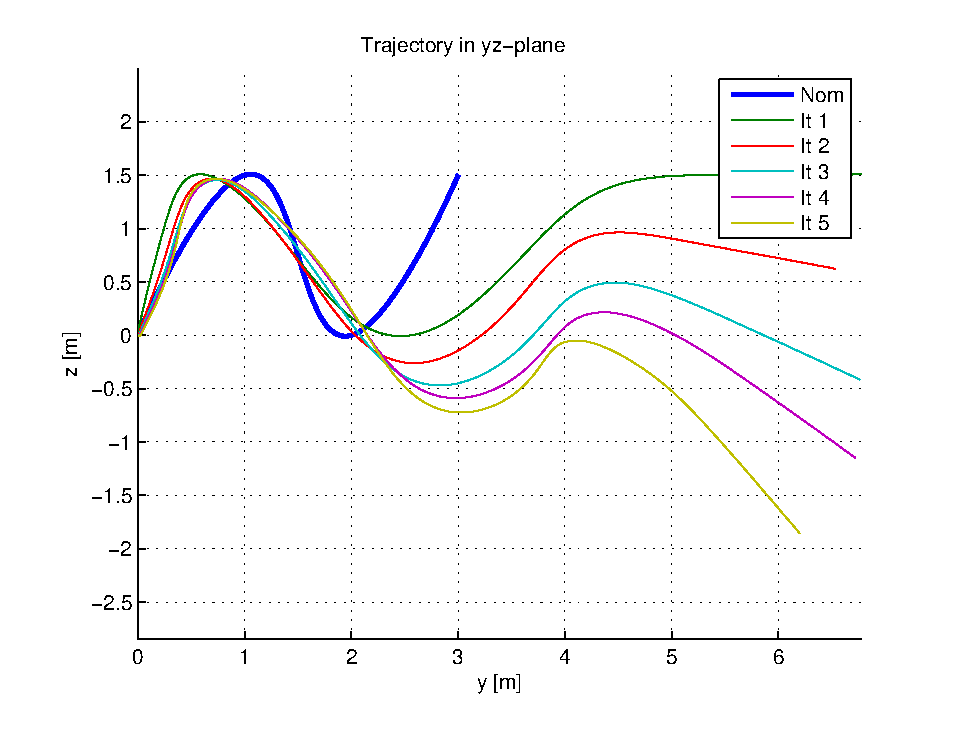
\includegraphics[scale=0.40]{ILCwind_yz.eps}			
\caption{ILC over iterations}
\end{figure}
\end{frame}
%
% End of slides
\end{document} 